% XCircuit output "lab4n.tex" for LaTeX input from lab4n.eps
\def\putbox#1#2#3#4{\makebox[0in][l]{\makebox[#1][l]{}\raisebox{\baselineskip}[0in][0in]{\raisebox{#2}[0in][0in]{\scalebox{#3}{#4}}}}}
\def\rightbox#1{\makebox[0in][r]{#1}}
\def\centbox#1{\makebox[0in]{#1}}
\def\topbox#1{\raisebox{-0.60\baselineskip}[0in][0in]{#1}}
\def\midbox#1{\raisebox{-0.20\baselineskip}[0in][0in]{#1}}
   \scalebox{1.08333}{
   \normalsize
   \parbox{7.45312in}{
   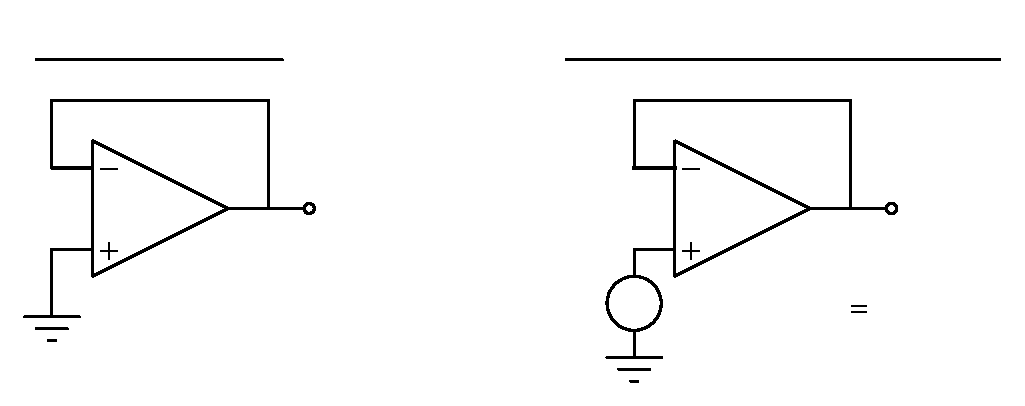
\includegraphics[scale=0.923077]{lab4n}\\
   % translate x=865 y=381 scale 0.41
   \putbox{0.22in}{2.11in}{1.20}{Follower Noise}%
   \putbox{3.47in}{2.11in}{1.20}{Follower Transfer Function}%
   \putbox{3.13in}{0.36in}{1.20}{AC 1}%
   \putbox{1.88in}{1.03in}{1.20}{$\overline{V_{o,loop}}^2$}%
   \putbox{5.47in}{1.03in}{1.20}{$V_o(f)$}%
   \putbox{4.63in}{0.45in}{1.20}{$|H(f)| = \frac{V_o(f)}{V_i(f)}$}%
   \putbox{3.13in}{0.61in}{1.20}{$V_i(f)$}%
   } % close 'parbox'
   } % close 'scalebox'
   \vspace{-\baselineskip} % this is not necessary, but looks better
